\documentclass[a4paper,13pt]{book}
\usepackage[centertags]{amsmath}
\usepackage{amscd}
\usepackage{amsthm}
\usepackage{amssymb}
\usepackage{enumerate}
\usepackage[dvips]{graphics}
\usepackage{graphicx, subcaption} % takes care of graphic including machinery
\usepackage{multicol}
\usepackage{hyperref}
\usepackage[english]{babel}
\usepackage{color}
\usepackage{tikz}
\usepackage{tabls} %per tenir m{\'e}s control sobre l'espai en les taules nom{\'e}s cal aquest paquet
\usepackage{indentfirst} %per comen\c{c}ar primer parragraf de seccio o capitol amb indent
\usepackage{imakeidx}
\makeindex

\usepackage[T1]{fontenc}
\linespread{1.1} % Palatino needs more leading (space between lines)

\usepackage[latin1]{inputenc}
\usepackage[twoside,bindingoffset=1cm]{geometry}


%%%%%%%%%%%%%%%%%%%%%%%%%%%%%%%%%%%%%%%%%%%%%%%%%%%%%%%%%%%%%%%%%%%%%%%%%
% theorem environments
%%%%%%%%%%%%%%%%%%%%%%%%%%%%%%%%%%%%%%%%%%%%%%%%%%%%%%%%%%%%%%%%%%%%%%%%%

\newtheorem{defn0}{Definition}[chapter]
\newtheorem{prop0}[defn0]{Proposition}
\newtheorem{thm0}[defn0]{Theorem}
\newtheorem{lemma0}[defn0]{Lemma}
\newtheorem{corollary0}[defn0]{Corollary}
\newtheorem{example0}[defn0]{Example}
\newtheorem{remark0}[defn0]{Remark}
\newtheorem{conjecture0}[defn0]{Conjecture}

\newenvironment{definition}{ \begin{defn0}}{\end{defn0}}
\newenvironment{proposition}{\bigskip \begin{prop0}}{\end{prop0}}
\newenvironment{theorem}{\bigskip \begin{thm0}}{\end{thm0}}
\newenvironment{lemma}{\bigskip \begin{lemma0}}{\end{lemma0}}
\newenvironment{corollary}{\bigskip \begin{corollary0}}{\end{corollary0}}
\newenvironment{example}{ \begin{example0}\rm}{\end{example0}}
\newenvironment{remark}{ \begin{remark0}\rm}{\end{remark0}}
\newenvironment{conjecture}{\begin{conjecture0}}{\end{conjecture0}}

\newcommand{\defref}[1]{Definition~\ref{#1}}
\newcommand{\propref}[1]{Proposition~\ref{#1}}
\newcommand{\thmref}[1]{Theorem~\ref{#1}}
\newcommand{\lemref}[1]{Lemma~\ref{#1}}
\newcommand{\corref}[1]{Corollary~\ref{#1}}
\newcommand{\exref}[1]{Example~\ref{#1}}
\newcommand{\secref}[1]{Section~\ref{#1}}
\newcommand{\remref}[1]{Remark~\ref{#1}}
\newcommand{\conjref}[1]{Conjecture~\ref{#1}}


%%%%%%%%%%%%%%%%%%%%%%%%%%%%%%%%%%%%%%%%%%%%%%%%%%%%%%%%%%%%%%%%%%%%%%%%%%%
%%%% local definitions for this paper
%%%%%%%%%%%%%%%%%%%%%%%%%%%%%%%%%%%%%%%%%%%%%%%%%%%%%%%%%%%%%%%%%%%%%%%%%%%

% monomio
\newcommand{\mono}{\texorpdfstring{\,\vcenter{\hbox{\includegraphics[scale=0.15]{./pictures/monomio/monomio.pdf}}}\,}.}

% dominoes
\newcommand{\VD}{\texorpdfstring{\,\vcenter{\hbox{
\includegraphics[scale=0.15]{./pictures/dominoes/v-domino.pdf}}}\,}i}
\newcommand{\HD}{\texorpdfstring{\,\vcenter{\hbox{\includegraphics[scale=0.15]{./pictures/dominoes/h-domino.pdf}}}\,}i}

% triminoes
\newcommand{\Itri}{\texorpdfstring{\,\vcenter{\hbox{\includegraphics[scale=0.15]{./pictures/trimonios/I3.pdf}}}\,}I}
\newcommand{\Ltri}{\texorpdfstring{\,\vcenter{\hbox{\includegraphics[scale=0.15]{./pictures/trimonios/L3.pdf}}}\,}L}


% tetrominoes
\newcommand{\OO}{\texorpdfstring{\,\vcenter{\hbox{\includegraphics[scale=0.15]{pictures/tetrominos/O.pdf}}}\,}O}
\newcommand{\TT}{\texorpdfstring{\,\vcenter{\hbox{\includegraphics[scale=0.15]{pictures/tetrominos/T.pdf}}}\,}T}
\newcommand{\LL}{\texorpdfstring{\,\vcenter{\hbox{\includegraphics[scale=0.15]{pictures/tetrominos/L_90.pdf}}}\,}L}
\newcommand{\LLvert}{\texorpdfstring{\,\vcenter{\hbox{\includegraphics[scale=0.15]{pictures/tetrominos/L.pdf}}}\,}L}
\newcommand{\JJ}{\texorpdfstring{\,\vcenter{\hbox{\includegraphics[scale=0.15]{pictures/tetrominos/J_90.pdf}}}\,}J}
\renewcommand{\SS}{\texorpdfstring{\,\vcenter{\hbox{\includegraphics[scale=0.15]{pictures/tetrominos/S.pdf}}}\,}S}
\newcommand{\ZZ}{\texorpdfstring{\,\vcenter{\hbox{\includegraphics[scale=0.15]{pictures/tetrominos/Z.pdf}}}\,}Z}
\newcommand{\II}{\texorpdfstring{\,\vcenter{\hbox{\includegraphics[scale=0.15]{pictures/tetrominos/I_90.pdf}}}\,}I}

\newcommand{\ALL}{\II, \allowbreak \OO, \allowbreak \TT, \allowbreak \SS, \allowbreak \ZZ, \allowbreak \JJ, \allowbreak \LL}


\NewDocumentCommand{\cell}{O{i} O{j}}{
 \langle #1, #2 \rangle
}
\NewDocumentCommand{\piece}{O{t} O{\theta} O{i} O{j} O{f}}{
 (#1, \allowbreak #2, \allowbreak \langle #3, \allowbreak #4 \rangle,  \allowbreak #5 )
}

\newcommand{\texttheo}[1]{\textnormal{\textsf{#1}}}
\newcommand{\tetris}[1]{\textsc{Tetris}[#1]\xspace}
\newcommand{\npc}{\textnormal{\textsf{NP-complete} }}
\newcommand{\pp}{\textnormal{\textsf{P}}}
\newcommand{\nph}{\textnormal{\textsf{NP-hard} }}
\newcommand{\survival}{$\texttheo{survival}$}
\newcommand{\clearing}{$\texttheo{clearing}$}


%%%%%%%%%%%%%%%%%%%%%% aixo pels headings %%%%%%%%%%%%%%%%%%%%%%%%
\usepackage{fancyhdr}
\pagestyle{fancy}
\renewcommand{\chaptermark}[1]{\markboth{#1}{}}
\renewcommand{\sectionmark}[1]{\markright{\thesection\ #1}}
\fancyhf{} \fancyhead[LE,RO]{\bfseries\thepage}
\fancyhead[LO]{\bfseries\rightmark} \fancyhead[RE]{\bfseries\leftmark}

\def\paginaenblanc{\newpage%
\thispagestyle{empty}%
\vspace*{2cm}%
\newpage%
\thispagestyle{empty}%
}


%%%%%%%%%%%%%%%%%%%%%%%%%%%%%%%%%%%%%%%%%%%%%%%%%%%%%%%%%%%%%%%%%%%%%%%%%
% aux commands
%%%%%%%%%%%%%%%%%%%%%%%%%%%%%%%%%%%%%%%%%%%%%%%%%%%%%%%%%%%%%%%%%%%%%%%%%
%==========================================================================
% macros to support private authors' notes
%==========================================================================
\newif\ifprivate
\privatetrue
\def\xbar{\vskip0.09in\hrule\vskip0.06in}
\def\private#1{\ifprivate \xbar {\em #1} \xbar
\else \fi}
\def\huh{\ifprivate ??? \marginpar{\Huge ???}
\else \fi}
\def\???{\ifprivate {\bf {???}} \marginpar{\begin{center}{\Huge {\bf ?}}\end{center}}
\else \fi}
%\def\???{\ifprivate {\bf {???}} \marginpar{{\Huge {\bf ?}}}
%\else \fi}
\marginparsep1mm
\def\nota#1{\ifprivate  $\clubsuit$ \marginpar{\parbox[t]{2.4cm}{\begin{center}\tiny #1\end{center}}}
\else \fi}
\def\comment#1{\ifprivate \marginpar{\parbox[t]{2.4cm}{\begin{center}\tiny #1\end{center}}}
\else \fi}
%\def\nota#1{\ifprivate  $\clubsuit$ \marginpar{\parbox[t]{1.8cm}{\tiny #1}}
%\else \fi}
\def\privateeject{\ifprivate\eject\fi}
%\def\???{{\bf {???}} \marginpar{{\Huge {\bf ?}}} }
%%%%%%%%%%%%%%%%%%%%%%%%%%%%%%%%%%%%%%%%%%%%%%%%%%%%%%%%%%%%%%%%%%%%%%%%%%

%%%%%%%%%%%%%% definicions cap{\'\i}tol ""%%%%%%%%
%%%%%%%%%%%%%%%%%%%%%%%%%%%%%%%%%%
\def\av{\underline{a}}

\def\Zr{\mathbb Z^r} \def\Nr{\mathbb N^r}
\def\xv{\underline{x}}
\def\yv{\underline{y}}
\def\zv{\underline{z}}

\newcommand{\Proj}{\operatorname{Proj}}
\newcommand{\Spec}{\operatorname{Spec}}


\def\HiRIM#1{H^i_{\mathcal M}(#1)}

\newcommand{\im}{\operatorname{Im}}
\renewcommand{\ker}{\operatorname{Ker}}
\newcommand{\grade}{\operatorname{grade}}
\newcommand{\Ext}{\operatorname{Ext}}
\newcommand{\Hom}{\operatorname{Hom}}
\newcommand{\m}{\mathfrak m}
\newcommand{\n}{\mathfrak n}
\newcommand{\M}{\mathfrak m}
%\newcommand{\cL}{{\mathcal L}}
\newcommand{\cP}{{\mathcal P}}
\newcommand{\cE}{{\mathcal E}}
\newcommand{\cS}{{\mathcal S}}
\newcommand {\PP}{\mathbb{P}}

\def\p{\mathfrak{p}}
\def\q{\mathfrak{q}}
\DeclareMathOperator{\de}{deg}

\DeclareMathOperator{\Hl}{H}
 \DeclareMathOperator{\h}{h}


%%%%%%%%%%%%%%%%%%%%%%%%%%%%%%%%%%%%%%%%%%%%%%%%%%%%%%%%%%%%%%%%%%%%%%%%
\begin{document}

\makeatletter
\def\old@comma{,}
\catcode`\,=13
\def,{%
  \ifmmode%
    \old@comma\discretionary{}{}{}%
  \else%
    \old@comma%
  \fi%
}
\makeatother

\section{Definitions}

Formalization of a Tetris game and definition of the problem. We will follow the definition from \cite{TIH}.


\begin{definition}
  A \emph{board} B is an $n$ by $m$ grid. Each cell $\cell$, $i = 1\dots n$, $j = 1\dots m$ is \emph{filled} or \emph{unfilled}.
\end{definition}

The board will be indexed from bottom to top and from left to right. The cell $\cell[1][1]$ is in the bottom left of the board and $\cell[n][m]$ is the top right-most cell. \\

The following definitions will define the pieces and how they interact with the board.

\begin{definition}
  A \emph{piece type} $t$ is one of the following:  \ALL. 
\end{definition}

\begin{definition}
 A \emph{piece state} in a board $B$ is a tuple $ P = \piece$ where:
  \begin{itemize}
    \item $t$ is a piece type
    \item $\theta$ is the \emph{orientation}, the number of degrees clockwise from the original piece. $ \theta \in \lbrace 0^\circ, 90^\circ, 180^\circ, 270^\circ \rbrace$
    \item $\cell$ is the \emph{position} of the piece in of $B$
    \item  $f$ indicates if the piece is \emph{fixed} or \emph{unfixed} in B.
  \end{itemize}

  We will refer to a piece sate as \emph{piece}.
   
\end{definition}

\begin{definition}
  Given a piece type $t$ and a board $B$, the piece $P_0 = \piece[t][0^\circ][n][\lfloor m / 2 \rfloor][\text{unfixed}]$ is the \emph{initial state} of the pice type of $t$ in the board $B$.
\end{definition}


The idea is to have only one active piece in a Tetris game. Only the piece that is moving has a state. When a piece reaches the \emph{fixed} state, is automatically merged with the board. Then the next piece starts in its initial state. In order to define how a piece moves thought the board, we need to define some \emph{moves} for changing the piece state.

\begin{definition}
  A \emph{rotaion model}
\end{definition}

VAL LA PENA DEFINIR EL CONJUT DE TOTS ELS ESTATS POSSIBLES?

\begin{definition}
  A \emph{move} is a computable function that changes the state of a piece under certain conditions. The following moves can be applied to a piece $P = \piece[t][\theta][i][j][\text{unfixed}]$. 
  \begin{itemize}
    \item \emph{clockwise rotation}
    \item \emph{counterclockwise rotation}
    \item \emph{slide to the left}
    \item \emph{slide to the right}
    \item \emph{drop by one row}
    \item \emph{fix}
  \end{itemize}
  If all the conditions are satisfied the move is said to be \emph{legal}, if any of the conditions are not satisfied the move is \emph{ilegal}. 
\end{definition}

Let's now define the \emph{trajectory} of a piece type in a Tetris game. Intuitively the trajectory starts when the piece is given to the player  and ends when he fixes the piece in the board.


\begin{definition}
 Let $B$ be a board and $t$ a piece type. Let $P_0$ be the initial state of the piece type $t$. Then a sequence of $k$ moves $\sigma = (m_1, ..., m_k)$ to the piece state after $i$ moves is a \emph{trajectory} if:

 \begin{itemize}
  \item the move $m_i$ over $P_i$ is a valid move for all $i = 1 \dots k$
  \item and $m_k$ is a \emph{fix} move.
 \end{itemize}
 
 Where $P_{i+1} = m_i(P_i)$ is the piece stat in $B$ after $i$ moves.
\end{definition}

After a piece trajectory a new board can be defined.

\begin{definition}
  Given a board $B$, a piece $p$ and some trajectory $t$, PRODUCTEd a new board $B'$ :wa:wa
\end{definition}

\chapter{Game variations}

A preliminary study on variants classifies different versions of the game into the following categories: limitations on player agility, piece set, losses, and rotation rules\cite{TIH}. Building upon this classification, we extend the previous work with the new definitions. The inputs for \textsc{Tetris} consist of the game board and the sequence of pieces. However, to fully define the problem, all other parameters must also be specified. Specifically, to define a game, we need to provide the polyominos that will appear, the available moves, and the initial state function.

In order to present all variations we will first define the basic Tetris, the problem presented in \cite{TIH}. Then a Tetris variation is the basic problem, but with some changes on the parameters. Two variations can be combined to produce a new one. Variations are grouped by the parameters they tweak.

We are introducing also some notation to define different Tetris games. 

\section{Basic Tetris}

The problem is:

$$\textsc{Tetris}\left[T_4,\varphi_0, \{s_l,s_r, r_+, r_-, d, f \},\Phi \right]$$

Let's break down the definition into parts. $T_4$ indicates that all the instances use the classic set of pieces, the ones made up by joining 4 blocks. $\varphi_0$ is the initial state function that places the pieces in the top-middle of the board. The available moves in each match are: slide to the left, slide to de right, rotate clockwise, rotate counterclockwise, drop by one row and fix a piece. 

For the objective function $\Phi$, \clearing\ or \survival\ will be both considered.


\section{Pieces Variations}

These variations modify the set of polyominos \( T \) used in the problem.

\begin{itemize}
  \item \( k\textsc{-tris} := \textsc{Tetris}[T = T_k] \)
  \item \( \leq k\textsc{-tris} := \textsc{Tetris}[T = T_1 \cup \dots \cup T_k] \)
\end{itemize}

The first variation replaces the classic \( T_4 \) polyominos with \( T_k \), the set of all \( k \)-ominos. The second variation utilizes all \( q \)-ominos up to \( k \). Additionally, we can consider variations that involve specific subsets of polyominos. For example, a variation that uses a subset of \( T_4 \) can be expressed as follows:

\[
\textsc{Tetris}[\{ \TT, \OO \}] := \textsc{Tetris}[T = \{ \TT, \OO \}]
\]

Representing the basic Tetris game, restricted to the tetrominos \( \TT \) and \( \OO \).


\section{Board Variations}

This variation imposes conditions on the valid board inputs. By restricting the set of board dimensions, new variations of the game emerge:

\begin{itemize}
  \item \( c\textsc{-column-Tetris} := \textsc{Tetris} \) where all input boards have \( c \) columns.
  \item \( r\textsc{-row-Tetris} := \textsc{Tetris} \) where all input boards have \( r \) rows.
\end{itemize}

In this context, \( c\textsc{-column-Tetris} \) and \( r\textsc{-row-Tetris} \) are subsets of the basic Tetris game, where the board width is fixed at \( c \) columns and the board height is fixed at \( r \) rows, respectively.

Additionally, we can impose conditions on the board's initial configuration. For example, we might require the board to be completely empty, with all cells unfilled:

\begin{itemize}
  \item \textsc{Empty-\textsc{Tetris}}: \textsc{Tetris} where all board cells are initially empty.
\end{itemize}

Another condition that could be imposed on the board is constructibility, as described earlier. It will be assumed that all boards are constructible.

\section{Moves Variations}

Move variations involve changes to the set of moves available in the game, ranging from rotating a piece to fixing it onto the board. These variations consist of adding, modifying, or removing moves from the standard set. Changes to the rotation functions, referred to as rotation variations, can include eliminating rotations entirely, such as:

\begin{itemize} \item $\textsc{Tetris-NoRotation} := \textsc{Tetris}[M = \{s_l, s_r, d, f\}]$ \end{itemize}

Alternatively, more complex rotation rules, such as Tetris standard SRS \cite{WikiFandom}, may be used. The aforementioned \emph{partial lock-out rule} is also a modification of the fix function, whic can be adjusted to either place the piece entirely within the board or fix it to just a single cell.

Other variations, for example, stem from the video game itself. In Tetris, especially during the early rounds, players can use the hard drop feature to avoid dropping a piece one row at a time. A hard drop moves the piece as far down as possible before it fixes into place. In this case, \emph{drop} and \emph{fix} are removed from the set of moves, and \emph{hard-drop} is introduced instead.

\begin{itemize} \item $\textsc{Tetris-HardDrop} := \textsc{Tetris}[M = { r_+, r_-, s_l, s_r, d_h }]$ \end{itemize}

This variations was first posted in \cite{TIH}. In some video game versions, players can set aside a piece for later use \cite{WikiFandom}. By adding a \emph{hold function} to the available moves, we can define a variant called \textsc{Tetris-WithHold}. However, this particular functionality will not be explored here.

\vspace{1em}


In the video game the pieces fall faster as the player fixes pieces. This causes that, in long matches, the player reaches a point where the pieces are pushed maximally downwards after each move. This behavior can be achieved by composing each function of the moves set with soft drop, so each time a move is done we ensure the piece is placed maximally downwards.   
\begin{itemize}
  \item $\textsc{Tetris-20G} := \textsc{Tetris}[\varphi = d_s \circ \varphi_0, M = d_s \circ M]$
\end{itemize}

The initial state function also is modified to ensure that the piece also is given to the player in the lowest possible possition. 

\section{Results}

With the problem and its variants presented, we present now the most relevant work around Tetris complexity. 
\textbf{COMENTAR CADA PROBLEMA ENFOCANT A "TROBAR LO QUE FA EL TETRIS COMPLICAT"}

In this section we resume the most relevant results, grouped by the paper in which they appear. They are sorted by publication date. 

\subsection{Tetris is hard, even to approximate}

The first results about Tetris complexity appear in \cite{TIH}. This result is about the corresponding of the decisional problems. For example the answer to \texttheo{height-filled} is the minimum $h$ such that $\texttheo{h-height-filled}$ holds.
\begin{theorem}
  Tetris is \nph to optimize (or approximate) with the objectives, \texttheo{cleared-rows}, \texttheo{tetrises} \texttheo{height-filled} and \texttheo{placed-pices}. It remains \nph even if:
  \begin{itemize}
    \item The player is restricted to two rotation/translation moves before each piece drops in height.
    \item Pieces are restricted to $\{\LL, \SS, \II, \OO\}$ or $\{\LL, \ZZ, \II, \OO\}$ plus at least one other piece.
    \item Losses are not triggered until after filled rows are cleared.
    \item Rotations follow any reasonable rotation model.
  \end{itemize}
\end{theorem}

\subsection{Total Tetris: Tetris with Monominoes, Dominoes, Trominoes, Pentominoes, ...}

In \cite{TT} a piece variation are explored. For $k \geq 1$ problems, k\textsc{-tris} and \textsc{NoRotation-}k\textsc{-tris}, with \survival\ and \clearing\ are all almost solved. For the basic problem, changing the polyominos set by increasing $k$ adds complexity to the polyminoes and increases the set size. Intuitively we can see that adding complex pieces to a game makes it more complicated. Results are presented in Table~\ref{tab:tt}.

\begin{table}[h!]
\centering
\begin{tabular}{|c || c | c || c | c ||} 
 \hline
  & \multicolumn{2}{| c ||}{\survival} & \multicolumn{2}{| c |}{\clearing} \\
 \hline
  & with rotation & no rotation & with rotation & no rotation \\
 \hline               
 $k = 1$ & \pp  & \pp  & \pp  & \pp \\ 
 \hline                             
 $k = 2$ & Open & Open & Open & \npc \\
 \hline                             
 $k = 3$ & Open & \npc & \npc & \npc\\
 \hline                             
 $k = 4$ & \npc & \npc & \npc & \npc\\
 \hline                             
 $k > 5$ & \npc & \npc & \npc & \npc\\
 \hline
\end{tabular}
\caption{\cite{TT} results with rotation}
\end{table}
\label{tab:tt}


\subsection{Tetris is NP-hard even with O(1) rows or columns}

In \cite{TCB} board variations are explored. These results help us get more intuition of Tetris complexity. Fixing the board size of the \textsc{Tetris} problem, in order to add complexity to the problem \textbf{TO FINISH:}.

\begin{itemize}
  \item \textsc{Empty $(\leq)k$-\textsc{tris}}: $(\leq)k$-\textsc{tris} where all the board cells are initially unfilled.
\end{itemize}

Results with this variation are in Table~\ref{tab:tcb}. 

\begin{table}[h!]
\centering
\begin{tabular}{|c | c | c | c | c |} 
 \hline
 Rows   & Columns & Empty  & Piece Sizes  & Complexity      \\
 \hline
 \hline
 $1   $ & $O(n) $ & no     & $O(n)    $ & strongly \nph   \\ \hline
 $1   $ & $O(n) $ & yes    & $O(n)    $ & linear          \\ \hline
 $1   $ & $O(n) $ & no     & $k       $ & linear          \\ \hline
 $2   $ & $O(n) $ & yes    & $O(n)    $ & strongly \nph   \\ \hline
 $3   $ & $O(n) $ & no     & $4       $ & Open            \\ \hline
 $4   $ & $O(n) $ & no     & $4       $ & strongly \nph   \\ \hline
 $O(n)$ & $1    $ & no     & $O(n)    $ & linear          \\ \hline
 $O(n)$ & $2    $ & no     & $O(n)    $ & polynomial      \\ \hline
 $O(n)$ & $3    $ & yes    & $O(n)    $ & strongly \nph   \\ \hline
 $O(n)$ & $3 - 7$ & no     & $4       $ & Open            \\ \hline
 $O(n)$ & $8+   $ & no     & $4       $ & strongly \nph   \\ \hline
 $O(n)$ & $8    $ & yes    & $\leq 65 $ & strongly \nph   \\
 \hline
\end{tabular}
\caption{\cite{TCB} results table}
\label{tab:tcb}
\end{table}

\subsection{Tetris with Few Piece Types}

In \cite{TWFP} they treat variations with fewer pieces, they only use a subset of the 7 available pieces types of Tetris. It uses the SRS rotation model.

\vspace{10px}

\textbf{Main Result:} for every 2-sized subset of $\{\ALL\}$, Tetris \survival\ and \clearing\ is \nph under SRS.

\vspace{10px}
\texttheo{20-G} and \texttheo{Hard-Drop} movement variations are introduced, and some results provided.

\vspace{10px}
\textbf{Result:} Tetris \texttheo{20-G} and Tetris \texttheo{Hard-Drop} is \npc  even if the pieces set is restricted to $\{ \II, \OO \}$ \cite{TWFP}. 


\textbf{Result:} if we allow the piece $\{ \TT \}$, the above result can be extended to \nph.



\section{Dominoes}

(Partial) lock rule? Constructible configurations. 

\subsection{Tetris with vertical dominoes}

Using the introduced notation, the problem is $\textsc{Tetris-NoRotation}\lbrack \VD \rbrack $ both  \clearing and \survival. The input consist of sequence of vertical dominoes and an arbitrary sized $n \times m$ board in a contractible configuration. The initial state function used in this variation differs since the default on the initial orientation, since the pieces must come in vertical orientation.

\subsubsection{Constructible board configurations}

First we will to characterize the constructible boards with $\VD$ pieces without rotation by exploring the configuration starting from an empty board. Vertical dominoes consist of two vertical adjacent cells. 

For an empty board, any trajectory fixes the piece in the bottom row, filling $\cell[1][i]$ and $\cell[2][i]$ cells for any $1 \leq i \leq m$. The next domino can either go to an empty column or to the one before. Placing the first $m$ dominoes in unfilled columns clears the two lowest rows, and consequently the board. When a domino is placed in a non-empty column $i$, the $\cell[3][i]$ and $\cell[4][i]$ are filled, and so on, util a $\VD$ is placed in the last unfilled column. When this happens the two lowest rows are cleared and the process continues. 

So we can represent a reachable configuration of a given $n \times m$ board $B$ with a sequence of $m$ integers $(a_1, \dots, a_m)$, where

$$0 \leq a_i \leq \lceil \frac{n}{2} \rceil, \;\;\;   \forall i = 1,\dots, m$$

and $\exists i$ such that $a_i = 0$ (an empty column), with the following mapping: 

$$
\cell = \begin{cases}
   \text{filled}  & \text{if } i \leq  2a_j  \\
   \text{empty}   & \text{if } i >  2a_j
\end{cases}
$$

Each $a_i$ counts the number of vertical pieces placed in the column $i$. For example, in a $10 \times 6 $  board, the sequence $(1,2,0,4,2,3)$ defines the configuration in 
\ref{dom:vconf}.

\begin{figure}[h]
    \centering
    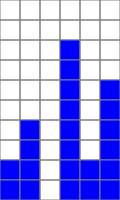
\includegraphics[width=0.2\textwidth]{./pictures/dominoes/vertical_configuration.pdf}
    \caption{The $10 \times 6 $ board configuration represented by the sequence $(1,2,0,4,2,3)$.}
    \label{dom:vconf} 
\end{figure}

\subsubsection{Cleaing}

In this decisional problem the input is a sequence of $k$ vertical dominoes and an $n \times m$ board with an initial configuration, that can be represented by the sequence $(a_1, \dots, a_m)$ as before. The question is: \emph{Is ther a way to clean the board after placing the $k$ pieces?}

\begin{theorem} 
$\textsc{Tetris-NoRotation}\lbrack \VD \rbrack $ \clearing is in \pp.
\label{dom:no-rot-vd}
\end{theorem}
\begin{proof}
    Let $B = (a_1, \dots, a_m) $ be the board representation and $k$ the length of the sequence of vertical dominoes. For every constructible board there is an empty column, so the strategy consists on placing each piece in an arbitrary empty column. 

    All the empty cells under the lowest empty row need to be filled to clean the board. Let $a_{\max}$ be the max in the board representation. Since we fill cells with dominoes, the number of dominoes $k_{\min}$ needed to clean the board is:
    $$ k_{\min} = \sum_{i = 1}^m \left( a_{\max} - a_i \right) $$

    If $k < k_{\min}$ we can't clear the board. If $k =  k_{\min}$ we can clear the board. And when $k > k_{\min}$, we can clean the board if after placing $k_{\min}$ dominoes the number of remaining pieces is a multiple of the board width, $k - k_{\min} \equiv 0 \mod m$. Since all the computations can be done in polyatomic time in respect of the input, the problem is in \pp.
\end{proof}

For boards with an even number of rows all pieces always fit inside the board. For an odd number of rows, dominoes could be placed in the top row with half of the domino inside the board and half outside. If we allow this, by changing the \emph{fix} function, the result would be the same since the same strategy works. The Figure~\ref{dom:vconf-filled} shows, in yellow color, how the number of pieces needed to clean the board are counted in Figure~\ref{dom:vconf}

\begin{figure}[h]
    \centering
    \includegraphics[width=0.2\textwidth]{./pictures/dominoes/vertical_configuration_filled.pdf}
    \caption{The $10 \times 6 $ board configuration needs 13 dominoes to be cleared.}
\label{dom:vconf-filled} 
\end{figure}


\subsubsection{Survival}

With the same input, the objective is to do not lose. The last proof provides a strategy to survive indefinitely. So for any number of pieces $k$ there is a way to avoid losing. Hence:
\begin{theorem} 
$\textsc{Tetris-NoRotation}\lbrack \VD \rbrack $ \survival is in \pp.
\end{theorem}


\subsection{Tetris with vertical dominoes}

As before, the problem is $\textsc{Tetris-NoRotation}\lbrack \HD \rbrack $ both \clearing and \survival. Placing a horizontal domino fills two adjacent cells in one row or clears the row. In any construtible board, each row has an even number of filled cells. When the board width is odd no row can be cleared, because to clear a row all the cells have to be filled. In this scenario the board can be cleared if the input consists on an empty board and an empty sequence of pieces. 

From now and on we assume the board has an even number of columns. Let $B$ be a board with $c$ columns. Let's divide the board in $c/2$ \emph{buckets}, a pair of consecutive columns. Then:

\begin{lemma0}   
    Not placing a domino inside a bucket makes the row unclearable.
\end{lemma0}
\begin{proof}
    Let $r$ be a row containing some dominoes. When a domino is placed in a bucket it divides the row into two parts: the cells on the left side of the domino and the ones on the right. Both parts of even length, and containing an even number of filled cells.

    In the other case the two parts have an odd length but containing an eaven number of filled cells, making them impossible to clean
    since there's no way to add an odd number of cells by placing dominoes.
\end{proof}

For example, in the Figure~\ref{dom:buckets}, the second piece occupies the second and the third bucket, making the row un-clearable. 

\begin{figure}[h]
    \centering
    \includegraphics[width=0.2\textwidth]{./pictures/dominoes/buckets.pdf}
    \caption{A board with one partially filled row.}
    \label{dom:buckets} 
\end{figure}

We now can prove both clearing and survival problems.

\begin{theorem}
    $\textsc{Tetris-NoRotation}\lbrack \HD \rbrack $ \clearing is in \pp.
\end{theorem}
\begin{proof}


    The input is an $n \times m$ input board $B$, filled with a construable configuration, and sequence of $k$ dominoes $\HD$. If $m$ is odd then the board can't be cleared if $k > 0$ or the initial board isn't empty. 

    When $m$ is even we first need to check if the board is clearable. If there's only one row, checking that the row has been built by placing each piece inside a bucket determines if the row is clearable. When the board has more than one row the same happens. 

    We first group in pieces the filled cells of each row from the initial board. This can always be done because there's no way to clean \emph{"half"} piece. Then we check if each piece is placed inside a bucket. If any piece isn't placed inside a bucket the board can't be cleared. We can compute this in $\mathcal{O}(n\cdot m)$.

    Now the board can be represented with a sequence $(a_1, \dots, a_{m/2})$ of $m/2$ numbers each representing the number of dominoes placed in each bucket. Let $a_{\max}$ be the maximum of the sequence. The minimum number of pieces needed to clear the board is:

    $$ k_{\min} = \sum_{i = 1}^{m/2} (a_{\max} - a_i )$$

    If $k < k_{\min}$ the board can't be cleared. If $k = k_{\min}$ the board can be cleard. When $k > k_{\min}$ the board can be cleared if $ k - k_{\min} \equiv 0 \mod m / 2$, we must ensure the remaining pieces to leave the board empty by filling rows.
\end{proof}

\begin{figure}[ht]
  \centering
  \begin{subfigure}[b]{0.3\textwidth}
    \centering
    \includegraphics[width=0.9\textwidth]{pictures/dominoes/horitzonatl_configuration_1.pdf}
    \caption{}
  \end{subfigure}
  \begin{subfigure}[b]{0.3\textwidth}
    \centering
    \includegraphics[width=0.9\textwidth]{pictures/dominoes/horitzonatl_configuration_2.pdf}
    \caption{}
  \end{subfigure}
  \begin{subfigure}[b]{0.3\textwidth}
    \centering
    \includegraphics[width=0.9\textwidth]{pictures/dominoes/horitzonatl_configuration_3.pdf}
    \caption{}
  \end{subfigure}
  \caption{Some board configurations. In (a) the board can't be cleared because the topmost domino is placed between the first and the second bucket. In (b) the board is represented by the sequence $(2,4,1,0,3)$, it can be cleared. The minimum number of pieces to clean the board is 10, this pieces apear in yellow in (c).}
  \label{dom:horitzonatl_configuration}
\end{figure}

Figure~\ref{dom:horitzonatl_configuration} shows some examples.

\begin{theorem}
    $ \textsc{Tetris-NoRotation}\lbrack \HD \rbrack $ \survival is in \pp.
\end{theorem}
\begin{proof}
    
    With the given board, we first find (???alortime???) a row to clear. If we find such a row we can survive indefinitely by repeatedly placing pieces in this row.

    If such a row doesn't exists, some dominoes can be placed inside board before a loss. To compute the maximum $k_{min}$(????)...

    If the input length is less or equal than $k_min$ we can survive, if not we can't.

\end{proof}


\section{Related problems}

Other problems related to Tetris.

\subsection{Tetris and decidability}

In \cite{TAD}, they consider a variant of Tetris where the sequence of pieces (together with their orientation and horizontal position, which cannot be changed anymore) is generated by a finite state automaton. They show that it is undecidable, given such an automaton, and starting from an empty game board, whether one of the generated sequences leaves an empty game board.

Since we are dealing with pieces sequences of a regular language we cannot fix the board height, so in this version the board height is unbounded. The formal problem definition is:

\vspace{1em}
\textbf{Instance:} an empty board $B$ of width $w$ and $L$, a regular language describing sequences of Tetris pieces with their initial position and orientation. 

\textbf{Question:} is there a sequence in $L$ that leaves the game board empty after dropping all pieces into the empty board?
\vspace{1em}

This problem with a board of width of 10 is undecidable for sequences only of $\II$ (reduction from PCP), but with only $\OO$ pieces the problem is decidable.


Introducing user intervention, letting the piece move while falling, we have the that the problem is decidable is the pieces types are restricted to $\{ \OO , \II \}$, or if the pieces are restricted to one piece type for arbitrary board width.

\subsection{Tetris is not Competitive}

Explores Tetris as an online game, where the player can only see the $l$-upcoming pieces (\emph{lock ahead}), in contrast with an offline game where the player knows completely the piece sequence.

In online-offline game studies, the goal is to compare an optimum offline strategy with an offline one. In this paper they construct pieces sequences without any loss-avoiding strategies for players with arbitrary (finite) lock ahead, but a loss-avoiding strategy exists in the offline version.

Next they use the before construction to show that an online player performs arbitrarily badly against an offline player for some optimization goals.

\subsection{How to construct Tetris configurations}

The main result of \cite{HTCT} is that every reasonable Tetris configuration is constructible, if a simple parity condition on the configuration is met.

To this problem we can attach a decision problem: given a configuration and an ordered series of Tetris pieces, their sizes satisfying a suitable congruence modulo 4; is it possible to construct the configuration using this series? 

We can also try to minimize the number of pieces needed to build a Tetris configuration.

\subsection{How Fast Can We Play Tetris Greedily With Rectangular Pieces?}

\cite{TWRP} considers a Tetris variant with a board of width $w$ a and an infinite height, where the pieces are rectangles of arbitrary integer dimensions and rotations are not allowed. The model definition is:

\begin{definition}[RDDS]
  A \emph{Rectangle Dropping Data Structure} maintains a set of $O(n)$ independent axis-aligned rectangles in the plane with integer coordinates, lying on or above the $x$-axis and between the vertical lines $x = 0$ and $x = w$, and allows the following:

  \begin{itemize}
    \item \emph{Preprocessing:} Initialize an empty RDDS containing no rectangle.
    \item \emph{Update:} Given an axis-aligned rectangle $R$ and a non-negative integer $x_d$, drop $R$ with left border at $x$-coordinate $x_d$ (here we assume that $R$ and $x_d$ are such that $R$ will lie between the lines $x = 0$ and $x = w$).
    \item \emph{Query:} Given an axis-aligned rectangle $R$, return the position where $R$ must be dropped to end up as low as possible (or one such position if it is not unique) as well as the height of the highest point in the set of rectangles which would result from that move.
  \end{itemize}
\end{definition}

RDDS is assumed to be a \emph{world-RAM machine}, an abstract machine similar to a random-access machine, but with finite memory and word-length. It works with words of size up to $ w $ bits, meaning it can store integers up to $2^{w} - 1$. 
The model is useful for analyzing the complexity of algorithms in a more realistic context, where the execution time not only depends on the amount of data but also on the representation of that data and the operations performed on it. 

They show that on a board with width $w = O(n)$, both operations of RDDS  cannot be supported in time $O(n^{1 / 2 - \epsilon})$ simultaneously if OMv (online matrix-vector multiplication problem) conjecture is true. 


\subsection{Why Most Decisions Are Easy in Tetris?}

Aquest mel vull llegir. Diu que el tetris no es especial.




\bibliographystyle{plain}
\bibliography{references} 

\printindex
\end{document}
